\documentclass[letterpaper,12pt,twoside,]{pinp}

%% Some pieces required from the pandoc template
\providecommand{\tightlist}{%
  \setlength{\itemsep}{0pt}\setlength{\parskip}{0pt}}

% Use the lineno option to display guide line numbers if required.
% Note that the use of elements such as single-column equations
% may affect the guide line number alignment.

\usepackage[T1]{fontenc}
\usepackage[utf8]{inputenc}

% pinp change: the geometry package layout settings need to be set here, not in pinp.cls
\geometry{layoutsize={0.95588\paperwidth,0.98864\paperheight},%
  layouthoffset=0.02206\paperwidth, layoutvoffset=0.00568\paperheight}

\definecolor{pinpblue}{HTML}{185FAF}  % imagecolorpicker on blue for new R logo
\definecolor{pnasbluetext}{RGB}{101,0,0} %


\usepackage{wrapfig,subcaption,array,tabularx} \captionsetup[figure]{font=scriptsize}

\title{QBUS2820 Assignment 1}

\author[]{}


\setcounter{secnumdepth}{0}

% Please give the surname of the lead author for the running footer
\leadauthor{}

% Keywords are not mandatory, but authors are strongly encouraged to provide them. If provided, please include two to five keywords, separated by the pipe symbol, e.g:
 

\begin{abstract}

\end{abstract}

\dates{This version was compiled on \today} 

% initially we use doi so keep for backwards compatibility
% new name is doi_footer

\pinpfootercontents{QBUS2820 Assignment 1}

\begin{document}

% Optional adjustment to line up main text (after abstract) of first page with line numbers, when using both lineno and twocolumn options.
% You should only change this length when you've finalised the article contents.
\verticaladjustment{-2pt}

\maketitle
\thispagestyle{firststyle}
\ifthenelse{\boolean{shortarticle}}{\ifthenelse{\boolean{singlecolumn}}{\abscontentformatted}{\abscontent}}{}

% If your first paragraph (i.e. with the \dropcap) contains a list environment (quote, quotation, theorem, definition, enumerate, itemize...), the line after the list may have some extra indentation. If this is the case, add \parshape=0 to the end of the list environment.


\hypertarget{introduction}{%
\section{Introduction}\label{introduction}}

Although the NBA is known for being a sport league across globe, it is a
vast economic entity as well. Undoubtedly, it has been a major impact in
the past decades, and it does not seem to be slowing down anytime soon.
Hence, economy is also a huge part of the business. Beside the League's
branding, its commercial success is contributed by the players at large
as they make the trends on social media and attract costumers to buy
their products in a constance. However, the most important attribute of
a player is none other than his performance on the court. Performance is
what NBA players thrive for as it decides their salary level. How much
salary a player is worth can be a hard estimation to the teams because
the performance of athlete fluctuates. Furthermore, the salary cap of
the League as a whole, too, fluctuate every year. Fortunately, the
League records players' data in various categories which include field
goal attempted, field goal percentage, offensive and defensive ratings,
etc. Data is a powerful tool because it can reflect a player's
contribution on the court with precision. Accompanied by the comparison
of the salaries given to a certain level of player, data can serve as a
strong reference that allows objective calculations.

This project aims to develop several predictive models of salary for NBA
basketball players. Three models including , k-nearest neignbour model,
a linear regression model and a lasso regression model are involved.

\textbf{summarizing findings}

\hypertarget{data-processing-and-exploratory-data-analysis}{%
\section{Data processing and exploratory data
analysis}\label{data-processing-and-exploratory-data-analysis}}

Two datasets \texttt{NBA\_train} and \texttt{NBA\_test} are analysed in
this project. The data is collected by NBA, with the corresponding raw
data and metadata being publicly accessible on the NBA websites.

There are 2 categorical variables and 19 numeric variables regarding
players' personal information and game performance, with an additional
unique ID of each record in the datasets. The numeric variables includes
salary, age, number of games played , number of minutes played, personal
efficiency rate , true shooting percentage, offensive rebounds ,
defensive rebounds , turnover percentage , assists , steals, blocks ,
turnover percentage , usage percentage , offensive rating, defensive
rating and win shares while the categorical variables are the position
and the team a player in.

The \texttt{NBA\_train} dataset is used for training and validating
predictive models in this project while the \texttt{NBA\_test} dataset
is used for testing selected models. Therefore the exploratory data
analysis is conducted based on the \texttt{NBA\_train} dataset.

Figure \ref{fig:correlation} illustrate that win share, defensive win
share, offensive win share, number of minutes played and personal
efficiency rate show linear relationships with salary, with win share
having the strongest linear relationship with salary at a correlation
coefficient of 0.68. It also provides evidences of linearity between
offensive win share, defensive win share and win share. Althought other
varables show mild linear relationship with salary, there can be other
linkage between salary and these variables. Thus variables showing no
linearity with salary can still be potentially informative and should be
left for further feature selection when developing predictive models.

\begin{wrapfigure}{l}{0.5\textwidth}
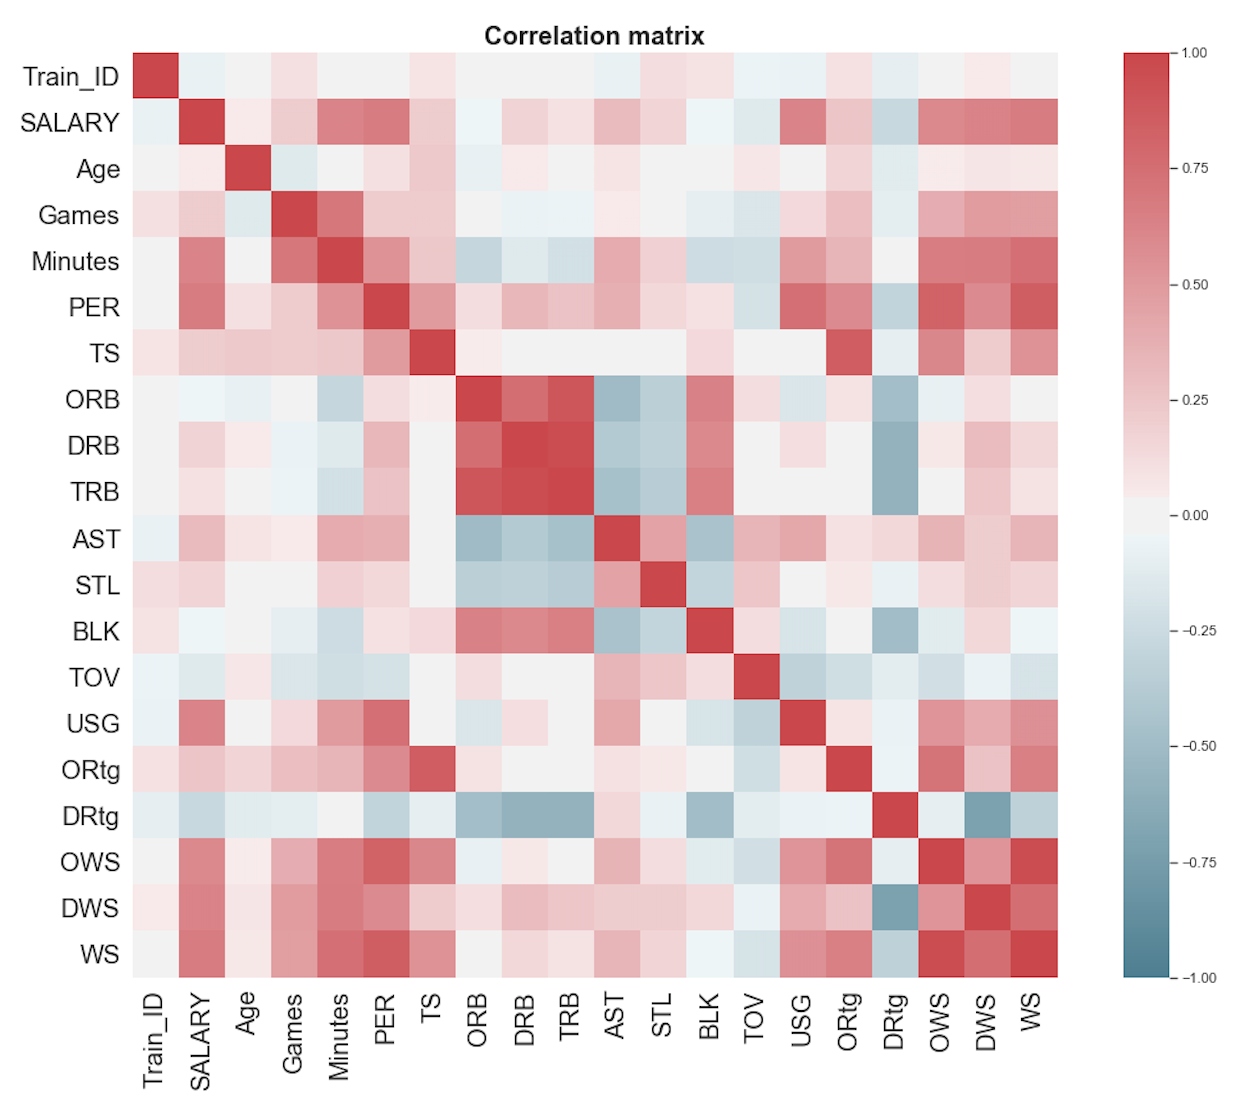
\includegraphics[width=0.8\linewidth]{correlation.png}
\centering
\caption{Correlations between numeric variables based on correlation coefficients.}
\label{fig:correlation}
\end{wrapfigure}

The relationships between salary and the six relative variables as well
as the distribution of numeric variables are further visualized by a
scatter plot matrix. In Figure \ref{fig:scatter}, the linearity between
numeric variables and salary shown is in line with the correlation
matrix (Figure \ref{fig:correlation}). Moreover, salary, win share,
defensive win share and offensive win share are significantly
right-skewed while usage percentage and personal efficiency rate are
slightly right-skewed. In additiona, the distributions demonstrates a
small variance of number of minutes played.

\begin{figure}[h]
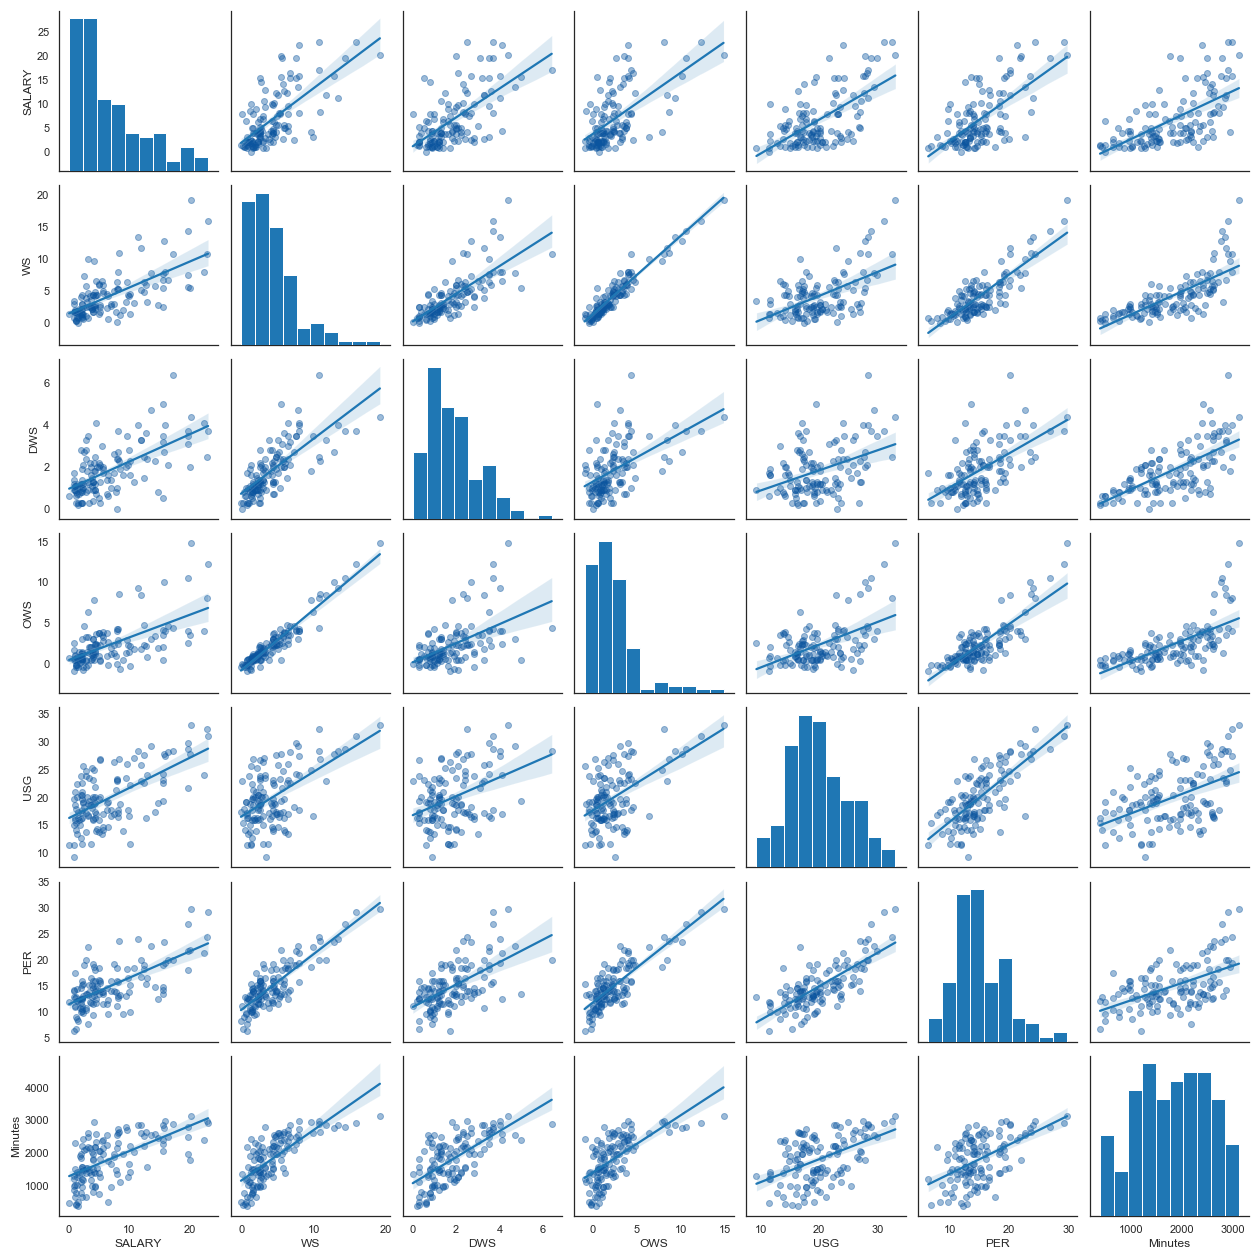
\includegraphics[width=0.8\textwidth]{scatter.png}
\centering
\caption{Distribution of numeric variables.}
\label{fig:scatter}
\end{figure}

To analyse the categorical variables, Figure \ref{fig:boxes} is
generated to visualise the distribution of salary. Figure
\ref{fig:position} describes how salary varies for players in different
positions. Although the median salaries are similar at \$4-6 millions
for the five positions, variances of salary are different. Salaries for
players in the center and small forward position vary significantly
without any outliers whereas variances of salary for both power forward
and shooting guard are much smaller with an outlier. As the
distributions of salary differ for different positions, the position a
player in could be the potential predictors of salaries.

Outlining in Figure \ref{fig:team}, salary varies across different
teams, which is reasonable in a business entity. There are many
basketball teams within the NBA, resulting in small sample sizes of
salary in each group. Some groups, such as Los Angeles Clippers, Phoenix
Surs and Denver Nuggets, have information of only one player being
recorded in this dataset, making the team variable uninformative.
Therefore, despite the different distributions of salary for players in
different teams, the team variable is not involved in development of
predictive models.

\begin{figure}[H]
\begin{subfigure}{0.5\textwidth}
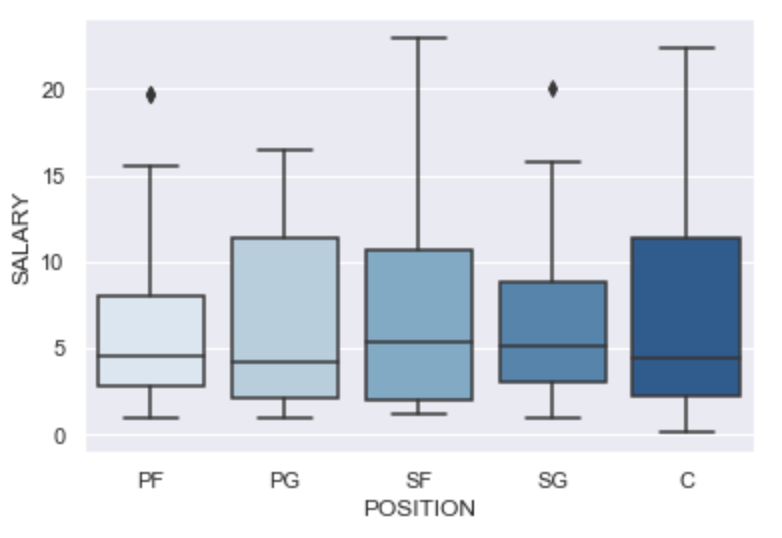
\includegraphics[width=0.9\linewidth, height=5cm]{position_box.png}
\centering
\caption{Salaries for players in different positions.}
\label{fig:position}
\end{subfigure}
\begin{subfigure}{0.5\textwidth}
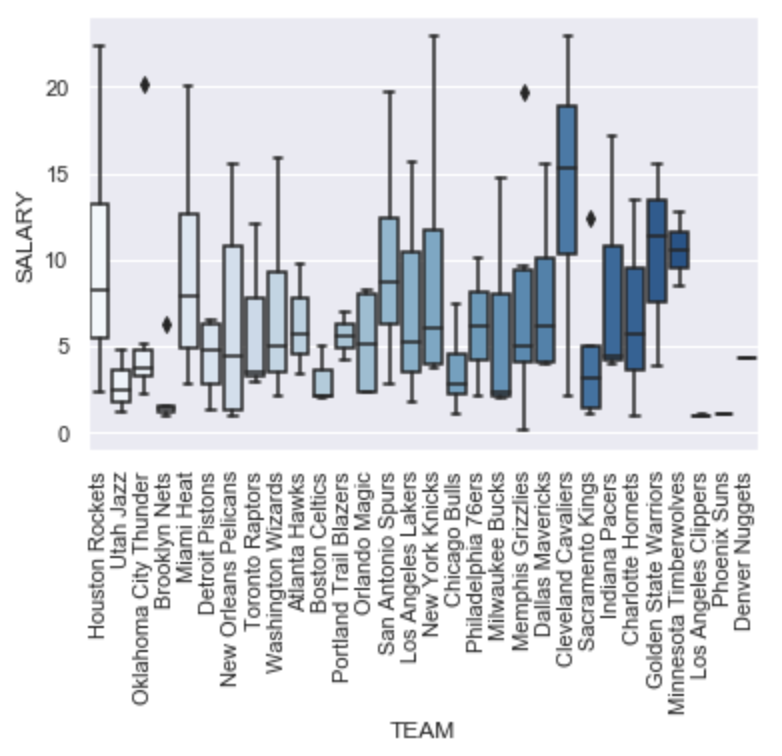
\includegraphics[width=0.9\linewidth, height=5cm]{team_box.png}
\centering
\caption{Salaries for players in different teams.}
\label{fig:team}
\end{subfigure}
\caption{Box plots of salaries for players in different teams and positions.}
\label{fig:boxes}
\end{figure}

\hypertarget{feature-engineering}{%
\section{Feature engineering}\label{feature-engineering}}

To discover any missing values involved in the datasets, bar charts of
missingness are generated to visualize missingness. As shown in Figure
\ref{fig:missingness}, both \texttt{NBA\_train} and \texttt{NBA\_test}
are complete without any missing values. Therefore no data removal or
data imputation is performed.

\begin{figure}[H]
\begin{subfigure}{0.55\textwidth}
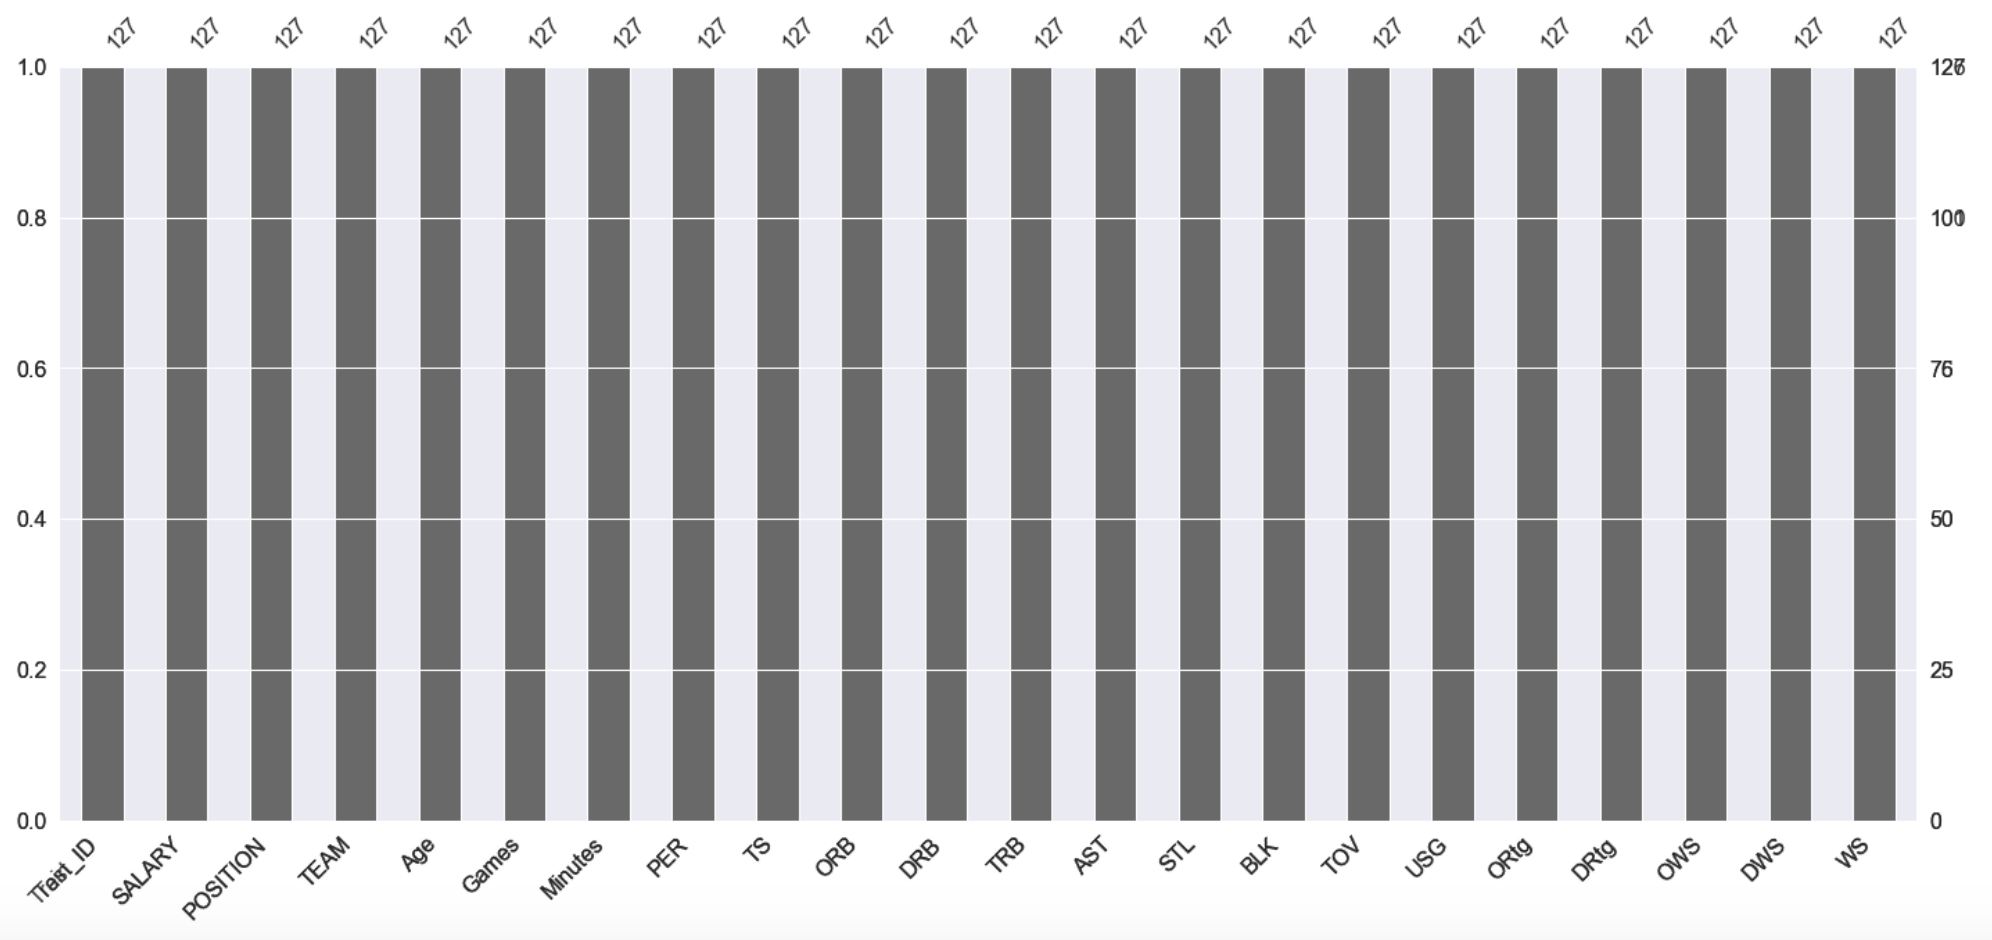
\includegraphics[width=0.9\linewidth, height=5cm]{nbaTrain_miss.png} 
\caption{Missingness bar chart of the `NBA train` dataset.}
\label{fig:trainMiss}
\end{subfigure}
\begin{subfigure}{0.55\textwidth}
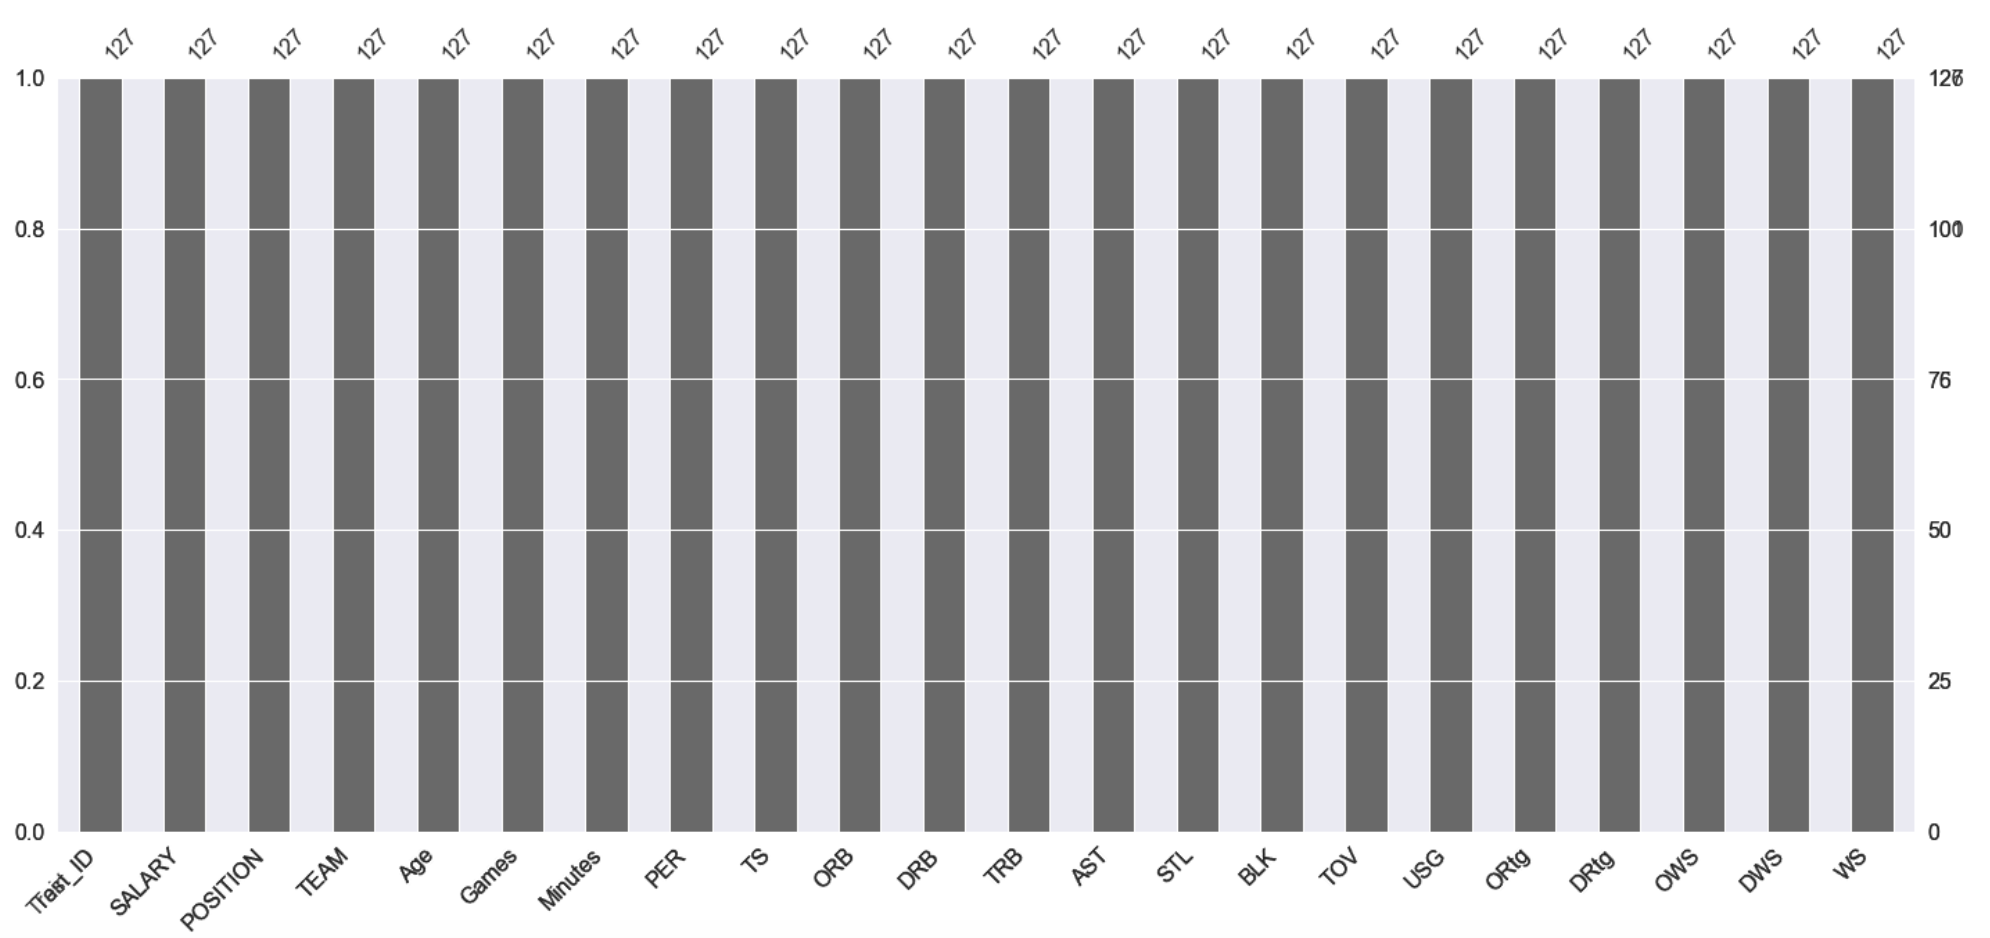
\includegraphics[width=0.9\linewidth, height=5cm]{nbaTest_miss.png}
\caption{Missingness bar chart of the `NBA test` dataset.}
\label{fig:testMiss}
\end{subfigure}
\caption{Visualizing the missingness of two datasets used.}
\label{fig:missingness}
\end{figure}

According to the results of exploratory data analysis, the record ID and
team played are uninformative for predicting salary. Therefore these two
variables are discarded whereas the salary is extracted from the
\texttt{NBA\_train} and \texttt{NBA\_test} datasets to be the response.
There are 19 numeric features and 1 categorical features, including age,
number of games played , number of minutes played, personal efficiency
rate , true shooting percentage, offensive rebounds , defensive rebounds
, turnover percentage , assists , steals, blocks , turnover percentage ,
usage percentage , offensive rating, defensive rating, win shares and
team the player in, remaining for predictive model development

In order to involve the categorical variable in predictive models, the
position played is encoded by a dummy variable whose values of
\texttt{1}, \texttt{2}, \texttt{3}, \texttt{4}, \texttt{5} represent
center(C), power forward(PF), point guard(PG), small forward(SF) and
shooting guard(SG) respectively.

After selecting and preprocessing the potentially informative features,
following the 80/20 rule, the \texttt{NBA\_train} dataset is splitted
into the training set and validation set. The training set is used to
develop models while the validation set helps to select models
developed.

\hypertarget{methodology-of-k-nearest-neighbour-regression-and-linear-regression-models}{%
\section{Methodology of K-nearest neighbour regression and linear
regression
models}\label{methodology-of-k-nearest-neighbour-regression-and-linear-regression-models}}

\begin{figure}[H]
\begin{subfigure}{0.5\textwidth}
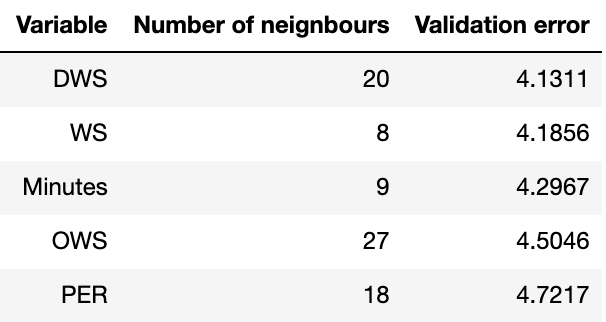
\includegraphics[width=0.9\linewidth, height=5cm]{knn_models.png} 
\caption{Top 5 K nearest neighbor models with the highest validation errors.}
\label{fig:subim1}
\end{subfigure}
\begin{subfigure}{0.5\textwidth}
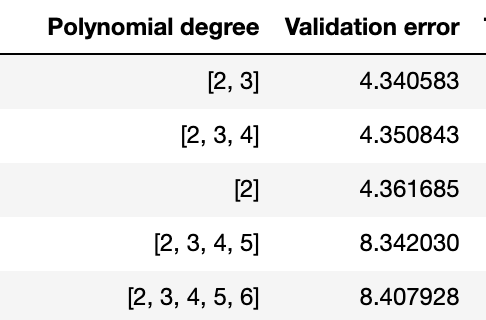
\includegraphics[width=0.9\linewidth, height=5cm]{poly_models.png}
\caption{Top 5 polynomial linear regression models with the highest validation errors.}
\label{fig:subim2}
\end{subfigure}
\caption{Validation errors of 10 models developed.}
\end{figure}

\hypertarget{methodology-of-the-model-that-is-not-covered-in-this-unit}{%
\section{Methodology of the model that is not covered in this
unit}\label{methodology-of-the-model-that-is-not-covered-in-this-unit}}

\hypertarget{test-set-performance}{%
\section{Test set performance}\label{test-set-performance}}

\hypertarget{analysis-and-conclusions}{%
\section{Analysis and conclusions}\label{analysis-and-conclusions}}

\hypertarget{appendix}{%
\section{Appendix}\label{appendix}}

\hypertarget{references}{%
\section{References}\label{references}}

\begin{itemize}
\item
  Bilogur, (2018). Missingno: a missing data visualization suite.
  Journal of Open Source Software, 3(22), 547,
  \url{https://doi.org/10.21105/joss.00547}.
\item
  NBA Stats. (2018). NBA Stats. {[}online{]} Available at:
  \url{https://stats.nba.com/}.
\item
  Rençberoğlu, E. (2019). Fundamental Techniques of Feature Engineering
  for Machine Learning. {[}online{]} Medium. Available at:
  \url{https://towardsdatascience.com/}.
\item
  Richards, J. (2020). Why We Use an 80/20 Split for Training and Test
  Data Plus an Alternative Method. {[}online{]} Medium. Available at:
  \url{https://towardsdatascience.com/}.
\end{itemize}

%\showmatmethods


\bibliography{pinp}
\bibliographystyle{jss}



\end{document}

